\section{Marco teórico}
El punto de partida del proyecto consta de una serie de tarjetas Zybo \hyperlink{3}{[3]} que incluyen la tecnología Zynq anteriormente citada, las cuales actuarán como nodos y que queremos conectar para realizar una comunicación entre ellas.

Dicha comunicación se establece para enviar un fichero entre ellas con el objetivo de recolectar una cierta información de cada una de ellas y enviarla al ordenador central.

\subsection{Tarjetas Zybo}
Las tarjetas Zybo o, también llamadas, placas de desarrollo, usadas en este proyecto, se corresponden con el modelo ``Zybo Zynq 7010'' (Figura \ref{Tarjeta Zybo Zynq 7010}) y pertenece a la marca DIGILENT$^{\circledR}$.

\begin{figure}[h]
	\centering
	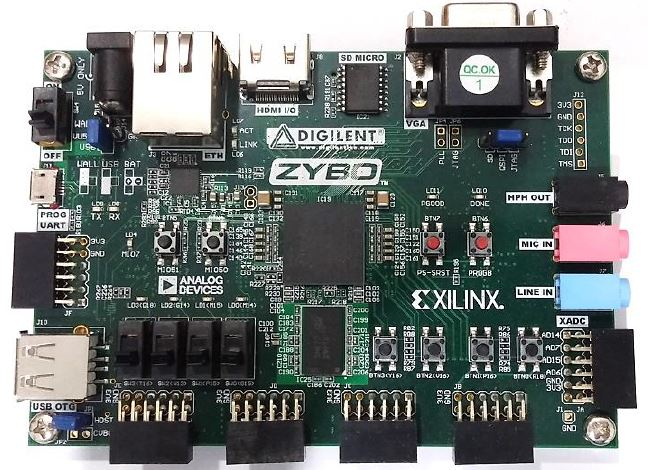
\includegraphics[scale=0.5]{Metodologia/MarcoTeorico/zybo.jpg}
	\caption{Tarjeta Zybo Zynq 7010}
	\label{Tarjeta Zybo Zynq 7010}
\end{figure}

Esta tarjeta está constituida por un software integrado con nivel de entrada listo para usarse y por una plataforma de desarrollo con un circuito digital de diversas características. Esta tarjeta de desarrollo pertenece a la familia Zynq de Xilinx, siendo el miembro de menor tamaño de la familia Zynq. \hyperlink{16}{[16]}.

\newpage
La Zybo Zynq 7010 está basada en la arquitectura de Xilinx ``All Programmable Sistem On Chip'' (ApSoC) completamente programable en la que se incluye un procesador de doble núcleo ARM Cortex A-9 con lógica Xilinx 7-series ``Field Programmable Gate Array'' (FPGA). Esta arquitectura la podemos ver en la Figura \ref{Arquitectura ApSoC de las tarjetas Zybo Zynq 7010}. \hyperlink{14}{[14]}.

\begin{figure}[h]
	\centering
	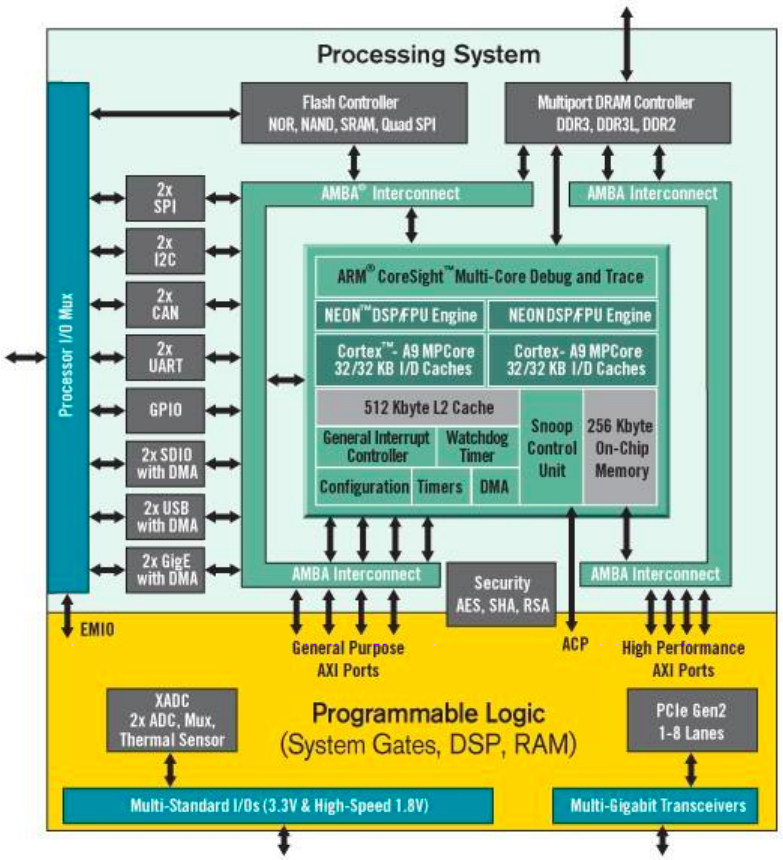
\includegraphics[scale=0.65]{Metodologia/MarcoTeorico/ApSoC.png}
	\caption{Arquitectura ApSoC de las tarjetas Zybo Zynq 7010}
	\label{Arquitectura ApSoC de las tarjetas Zybo Zynq 7010}
\end{figure}

Una particular característica de estas tarjetas de desarrollo es que su diseño no necesita de un hardware adicional pues ésta incluye las memorias en placa, E/S de vídeo y audio, USB, Ethernet y ranura para tarjeta SD de doble función. También es compatible con la nueva Suite de diseño de Vivado de alto rendimiento de Xilinx así como el conjunto de herramientas ISE/EDK. \hyperlink{14}{[14]}.

Estas características permiten que los proyectos que se quieran realizar sean más sencillos y visuales con el manejo de la FPGA integrada en la tarjeta gracias al procesador ARM manejado a través de un sistema operativo. Esto nos permite diseñar y manejar un sistema completo. \hyperlink{14}{[14]}.

La tarjeta Zybo Zynq 7010, con su tecnología ApSoC tiene su maestro de estructura en el procesador que también controla el resto de periféricos del sistema de procesamiento. \hyperlink{14}{[14]}.



Gracias a la tecnología Zynq usada, podemos abordar aplicaciones del sistema con tecnología de gama alta, por ejemplo video-vigilancia, asistencia automotriz-conductor, etc. La mayor característica de la arquitectura Zynq es pasar de una plataforma de FPGA centrada a un modelo de procesador céntrico que, en la arquitectura Zynq anterior, no estaba aplicado. \hyperlink{15}{[15]}.

Para los desarrolladores de software, dicha tecnología parece lo mismo que un procesador estándar, totalmente basado en ARM y SoC, arrancando de inmediato en el encendido y capaz de ejecutar una variedad de sistemas operativos con independencia de la lógica programable. \hyperlink{15}{[15]}.

El procesador ARM Cortex A-9 incorporado en las tarjetas de desarrollo Zybo Zynq 7010 tiene las siguientes características \hyperlink{17}{[17]}:
\begin{itemize}
	\item Doble núcleo a 650 MHz.
	\item Conjunto de extensiones NEON SIMD capazde realizar hasta 16 operaciones por instrucción.
	\item Alto rendimiento en unidades de coma flotante duplicando el rendimiento de las FPU anteriores de ARM.
	\item Extensiones de seguridad.
	\item Controlador de memoria caché L2 (0-4 MB).
\end{itemize}

Dichas características, son las que nos permiten la ejecución de sistemas operativos para poder controlar de una forma más rápida y sencilla, todos los periféricos de la tarjeta, incluyendo su FPGA.